\documentclass[11pt]{article}
\usepackage[utf8]{inputenc}
\usepackage{amsmath,amssymb}
\usepackage{graphicx}
\graphicspath{ {./images/} }
\usepackage[margin = 1.2 in]{geometry}
\usepackage{titlesec}
\usepackage{textcomp}
\usepackage{sidecap}
\usepackage{verbatimbox}
\sidecaptionvpos{figure}{t}
\usepackage{wrapfig}
\usepackage[margin=0cm]{caption}
\captionsetup[figure]{labelfont={bf},name={Figure},font=footnotesize}
\usepackage{multicol}

\begin{document}
\begin{titlepage}
    \title{\vspace{40pt}\Huge KiriZen: Creation of an iPhone application in swift based on the art of kirigami}

    \author{ \\\hline \\\\\\ \Large \vspace{5pt} Author: Stephanie Tindal \\\Large \vspace{5pt}{Student ID: 1936508}\\\Large \vspace{50pt}{Supervisor: Achim Jung} \\ \hline\\\\\\  \vspace{5pt}{MSc Computer Science} \\ \vspace{5pt}{School of Computer Science, University of Birmingham}\\\\\\ \hline\\\\}

    \date{September 2019 \vspace{20pt}}
    \maketitle
\end{titlepage}
\begin{frame}{}
    \begin{multicols}{2}
    \tableofcontents

\end{multicols}
\end{frame}

\newpage

\begin{abstract}
    Abstract abstract 

\end{abstract}

\vspace{50pt}
\renewcommand{\abstractname}{Acknowledgements}
\begin{abstract}
    I would like to thank Professor Achim Jung for supervising me throughout the project and Dr Iain Styles for the initial idea of an origami based application. 
\end{abstract}

\newpage
\section{Introduction}

        \subsection{A Brief History of Origami and Kirigami}
        
            \paragraph{}
            Origami is the art of folding paper. One of its earliest depictions was the folding of an ancient Egyptian map made from papyrus. Upon the invention of paper, paper folding was used mainly in religious ceremonies due its high price. There are examples of paper folding across many cultures therefore it is difficult to say where and when it was invented. In japan paper folding was popularised 
            % \cite{origami bible stuff}
            kirigami
            in Japanese, "kiri" means "to cut"
            \cite{Temko2004kirigami}
          
            Kirigami in addition to origami includes cutting the paper. 2 
            Houdini 
    
            \subsubsection{Relevance}
                \paragraph{} 
                Although paper folding used to be used in mostly religious contexts, origami has become more recreational in nature. 
            
                \paragraph{} 
                Origami and kirigami are now seen in pop-culture and art galleries. 
                %star wars
                %fashion
                %articles
                %books
                I learnt origami and kirigami from Chinese and Japanese students my grandmother hosted when I was younger and remember searching for books in the UK but not being able to find them in any libraries in my hometown. Now these types of books are widely available in most bookshops and libraries sometimes which entire sections dedicated to them. This increase in popularity or origami and kirigami.
            
                In addition to this,  origami and kirigami 
            
            
                % \cite{origami bible stuff}
    
                In recent years
            
                relaxation and mindfulness activities and applictions growing in popularity and including all ages such as adult colouring books, origami packs, head space applicatoin, 
                
        
        \subsection{Idea Conception}
            
                    \paragraph{} 
                        Having been a keen creator of origami from the age of 4, it was suggested by one of my professors that I create an application that involves origami. Upon discussion with my supervisor we decided to focus on kirigami - a branch of origami which involves cutting as well as folding the paper. The decision was made to have two aspects of the app - creation 
                        as discussed above, the popularity of kirigami is growing as is the popularity of relaxing head space apps. I only found a handful of apps focused on origami or kirigami on the app store that were not tutorials - discussed in section 2 - therefore I believe there is a place for the app I have created. so the market is not over saturated. 
        
                \subsection{Project Aim}
            
                 \paragraph{} 
                 The aim of the project is to create an application in which users can create cuts in a virtually folded sheet of paper and the application will reveal the unfolded pattern to them upon the click of a button. The application will 
                 
                 
                 The next level will allow the users to try and imagine how to cut the shape that is shown from the folded piece of paper.

The application will have to be virtually appealing and


• Relevance: The app will allow users to train their 3D imagination by interacting with the application. 

In addition to the application itself, users can mimic the patterns created in real life increasing their creativity.

                 1. Learn the basics for creating an iPhone application
2. Create an application for iPhone that allows the user to draw cuts into a folded piece of
paper
2.1. Demonstrate a crease pattern and folding of a square piece of paper into 2
2.2. Allow the user to draw cuts into the piece of paper
2.3. Reveal the image of the paper unfolded with the cuts made
2.4. Repeat for folding the square into 4, 6 (as you cannot fold a piece of paper into 3 or
5 layers about a central point) – revealing the unfolded cut versions at the end.
3. Add another level to the application which has an unfolded target shape and asks you what cuts are to be made to create this shape. E.g. pentagon is the target shape. The
application reveals the square folded into 5 and asks you where the cut should be made. 3.1. A margin of error will have to be programmed into this.
3.2. Application will show you the solution once you have tried.
4. Additional features
4.1. Additional features can be programmed for example changing the colours and
shading.
4.2. Higher number of folds.
4.3. Showing the actual folding/unfolding of the piece of paper in between steps
                 
            \subsection{Swift}
               
                \paragraph{} 
                    To create an iPhone application, swift is the most common language to use.  the iPhone decided to use swift so I can create the application on my iPhone and was looking forward to the challenge of a new language. Xcode is the integrated development environment (IDE) used for swift - the main language used to create iPhone applications. A beta version of this software is available for developments which contains extra however I decided to not use the beta version as while reading about them online I discovered they tend to have a lot more bugs. They are generally used by developers to so I would consider using it in a future application to have the most up to date software.

\newpage
\section{Background Research}

        \subsection{Kirigami-like Applications}
           \paragraph{}
            I searched for applications on the web and iPhone app store with a theme that centered around creating kirigami. I wanted to gain an insight into what is already out there to make sure my idea was unique, and to evaluate the strengths and weakness of the other apps as a user and learn from them before I design my own app. 
        
            \subsubsection{Paper Snowflake Maker}
            
                \paragraph{Type:} Web application %\cite http://rectangleworld.com/PaperSnowflake/
                
                \paragraph{Description:}
                Paper Snowflake Maker is a website where the user can cut out polygons from the shape of a ready folded piece of paper (the panel on the right of \textbf{Figure~\ref{fig:paperSnowflakeMaker}}) by clicking on the screen to make the corners of the polygon. The paper snowflake is virtually created and revealed to the user (left panel of \textbf{Figure~\ref{fig:paperSnowflakeMaker}}).
                
                    \begin{figure}[ht]\centering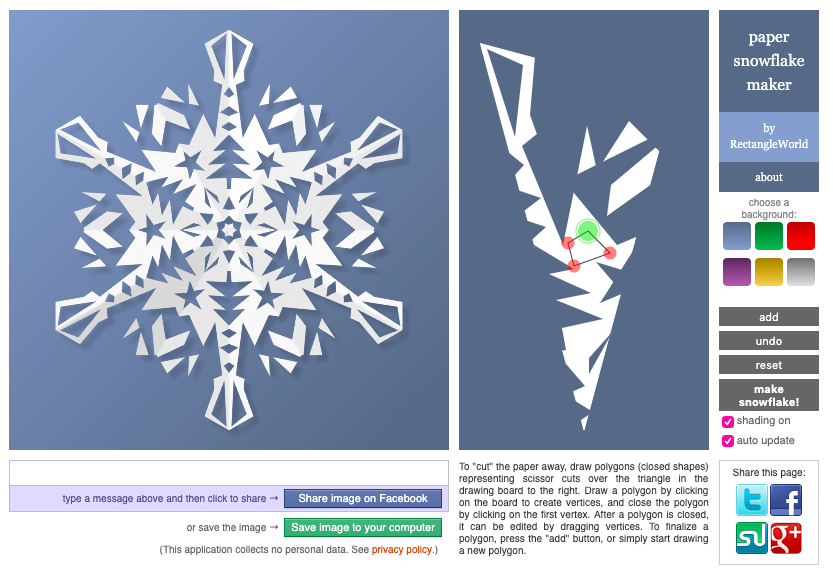
\includegraphics[width=0.9\textwidth]{Images/paperSnowflakeMaker}
                        \caption{
                        \label{fig:paperSnowflakeMaker}
                        A full page screenshot taken from the web application Paper Snowflake Maker. The user has made cuts on the folded image and is about to complete their next cut. The green dot indicated the beginning of a cut, the red dots indicate the corners of the polygon to be cut. When the users mouse passes over the green dot - an additional circle is created around its edge indicating to the user that if they click there, the polygon they created will be cut from the virtual piece of paper. The corners of the polygon can be dragged to a different shape before the cut is finalised.}
                    \end{figure}
                    
                \paragraph{Strengths:}
                It is clear how to make cuts in the virtual folded piece of paper as soon as you start clicking on it, as seen on the right panel in \textbf{Figure~\ref{fig:paperSnowflakeMaker}}. The green and red dots that appear as you click are clear indicators for the progression of the cut.
                
                The auto update button is a convenient feature as the user does not have to click the "make snowflake!" button every time a new shape is cut. The draggable corners are an additional convenient feature if the user would like to edit the shape of the polygon before the cut is created.
                 
                 The shading of the final snowflake provides a sense of realness as its shadows appears as a folded pieces of paper would.
                 
                \paragraph{Weaknesses:}
                When using the application the add button (which finalises the cut - mostly meaning the construction lines on the folded paper image are removed) seems unnecessary as it has the same functionality as other actions like starting to draw a new shape, or clicking the "make snowflake!" button.
                
                The cuts that can be made on this virtual snowflake are much more complex than those which can recreated on a real piece of paper, this taking away from the sense of realism slightly. The smaller pieces that are created in \textbf{Figure~\ref{fig:paperSnowflakeMaker}} would fall off after being severed from the main larger component also contrasting the realism.
                
                The save image to your computer button opens another window explaining how to save the image and ironically does not allow you to save the image to your computer. Copying the image produced a low resolution image as does saving the image straight from the original screen. In addition the "share image on Facebook button does not work."
                
                \paragraph{Lessons Learned:}
                The cutting is intuitive for this web application - I can consider this approach when developing my own. The overall look of the images is clean, however the buttons on the side and instructions could be updated for a more modern feel. Buttons that do not provided the intended functionality should be discarded.
                
            \subsubsection{Snowflake!}
            
                \paragraph{Type:} iPhone application 
            
                \paragraph{Description:}
                Snowflake is an application that allows the user to cut out free-form shapes from either 22.5\textdegree{} segments or 45\textdegree{} segments. The image revealed is created from combining copies of the segment to complete the snowflake-like shape shown in \textbf{Figure~\ref{fig:snowflakeResult}} which is created from the 22.5\textdegree{} segments from \textbf{Figure~\ref{fig:snowflakeSegmentCut}}. 
                    
                    \begin{figure}[!ht]
                        \begin{minipage}{0.45\textwidth}
                            \centering 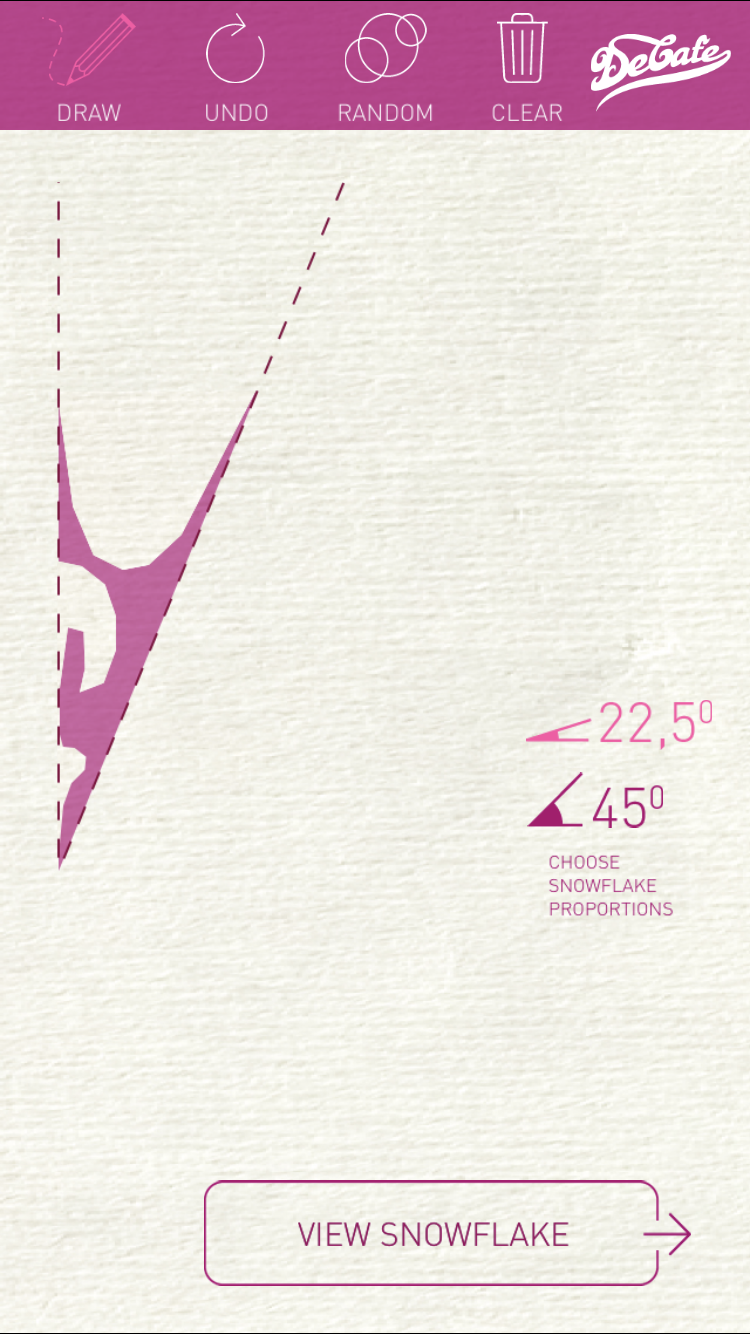
\includegraphics[width=0.7\linewidth]{Images/snowflakeSegmentCut}
                            \caption{A ready made cut resulting from the press of the "Random" button. The segment size selected is 22.5\textdegree{}. Pressing the "View Snowflake button takes the user to \textbf{Figure~\ref{fig:snowflakeResult}} screen.\\}
                            \label{fig:snowflakeSegmentCut}
                        \end{minipage}\hfill
                        \begin{minipage}{0.45\textwidth}
                            \centering
                            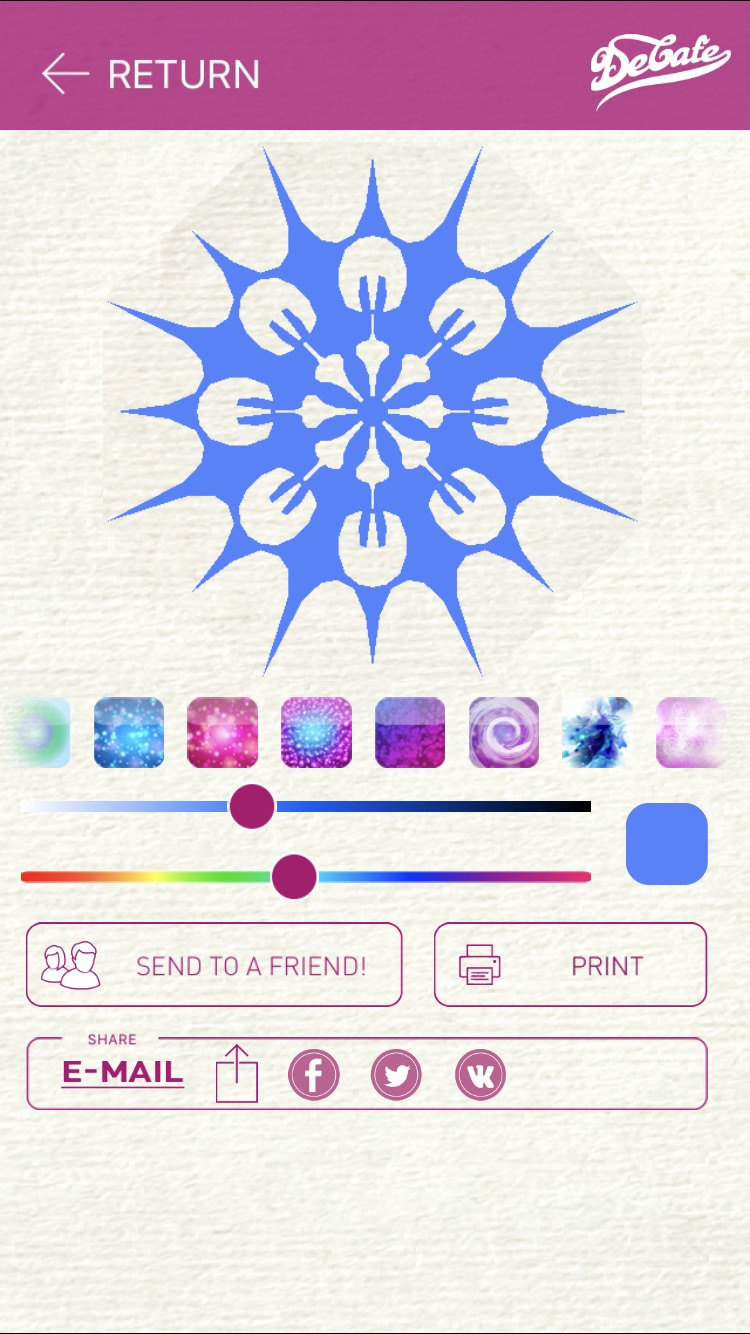
\includegraphics[width=0.7\linewidth]{Images/snowflakeResult}
                            \caption{The result of the cut made in \textbf{Figure~\ref{fig:snowflakeSegmentCut}}. The colour of the image can be altered with the colour pickers below it. The image can be shared with the buttons in the "Share" section providing the relevant button works.}
                            \label{fig:snowflakeResult}
                        \end{minipage}
                    \end{figure}
                    
                    
                    
                \paragraph{Strengths:}
                A version of Tchaikovsky's Dance of the Sugar Plum Fairy plays in the background which is synonymous with Christmas an in keeping with the theme of the application. 
                The user can use the random shape button to create a base to start with. 
                
                \paragraph{Weaknesses:}
                Snowflakes have six sides due to the shape of the H\textsubscript{2}O molecule. Eight sided crystals would never be formed naturally %\cite{http://www.its.caltech.edu/~atomic/snowcrystals/unusual/unusual.htm} 
                therefore it is an odd choice for this application to choose pieces of paper folded into segments with angles of 22.5\textdegree{} and 45\textdegree{}, as this forms 8 or 16 sided snowflakes rather than the more common 6 or at most 12 sided snowflakes.
                
                The area of the screen dedicated to the main function of creating cuts from a segment of the final shape consists of a very small portion of the screen. The ratio is especially low when cutting from the 22.5\textdegree{} segments as seen in \textbf{Figure~\ref{fig:snowflakeSegmentCut}}.
                
                The shape that is cut from the shape drawn is not always as expected. For example in \textbf{Figure~\ref{fig:snowflakeSegmentCut}} this does not reflect the cut you would expect from the free-form shape drawn by the user in \textbf{Figure~\ref{fig:snowflakeOutline}}.
               
                On the share bar seen in the centre of \textbf{Figure~\ref{fig:snowflakeResult}}, the "Send to a friend!" button has exactly the same response as the "E-Mail" button. It is also slightly  misleading as I would expect this button to create a message via WhatsApp or iMessage rather than email if sending to a friend. The upload icon button allows the user to create a "Happy new year" themed postcard and when the "Send" button is pressed, the pop-up disappears leaving the user with no idea where the image they just created was saved or sent unlike with the buttons that do work - the user is sent to the relevant email or social media screen. The same situation occurs when the twitter button (icon of a bird) is pressed - no response occurs after the "Send" button is pressed.
                
                The status bar disappears on the app so the user is not able to see information such as signal, battery life time etc while using the application. 
                 
                 \begin{figure}[!ht]
                        \begin{minipage}{0.45\textwidth}
                            \centering 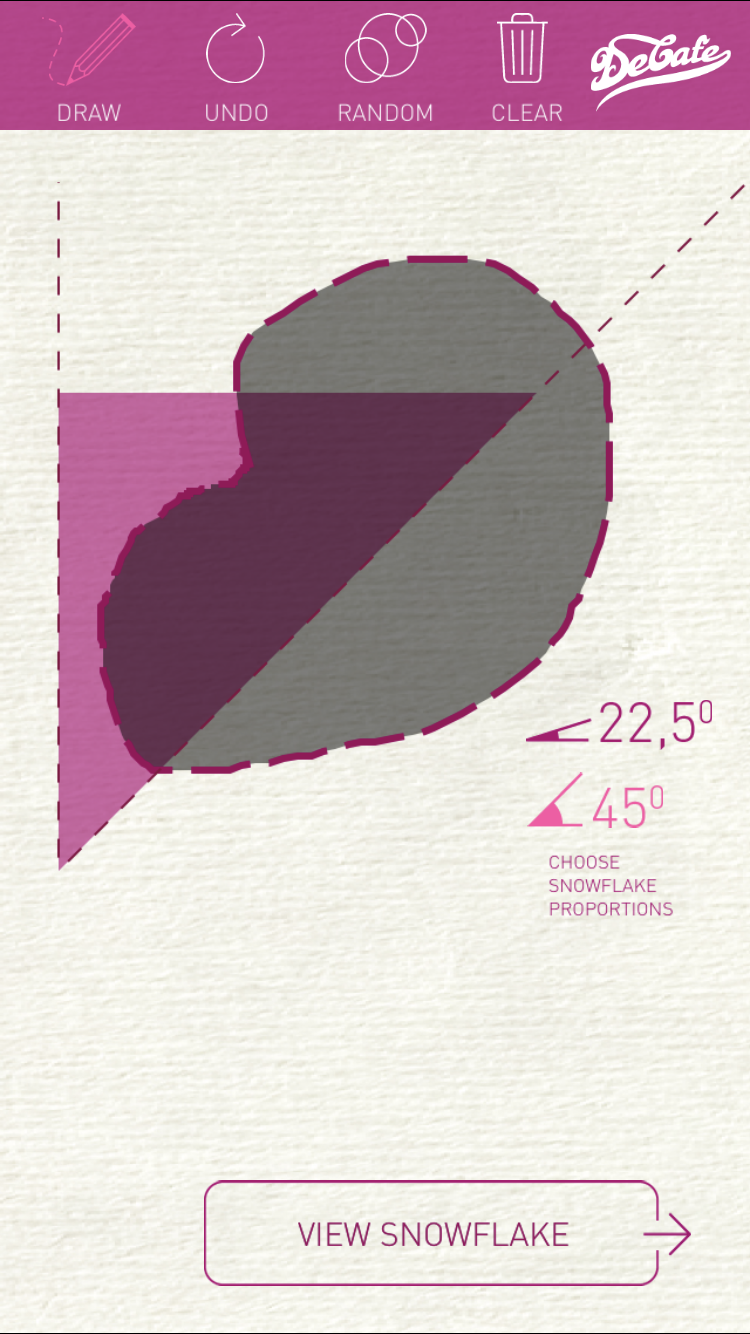
\includegraphics[width=0.7\linewidth]{Images/snowflakeOutline}
                            \caption{A free-form line is drawn on a 45\textdegree{} segment to indicate where the user has drawn the cut.\\\\}
                            \label{fig:snowflakeOutline}
                        \end{minipage}\hfill
                        \begin{minipage}{0.45\textwidth}
                            \centering
                            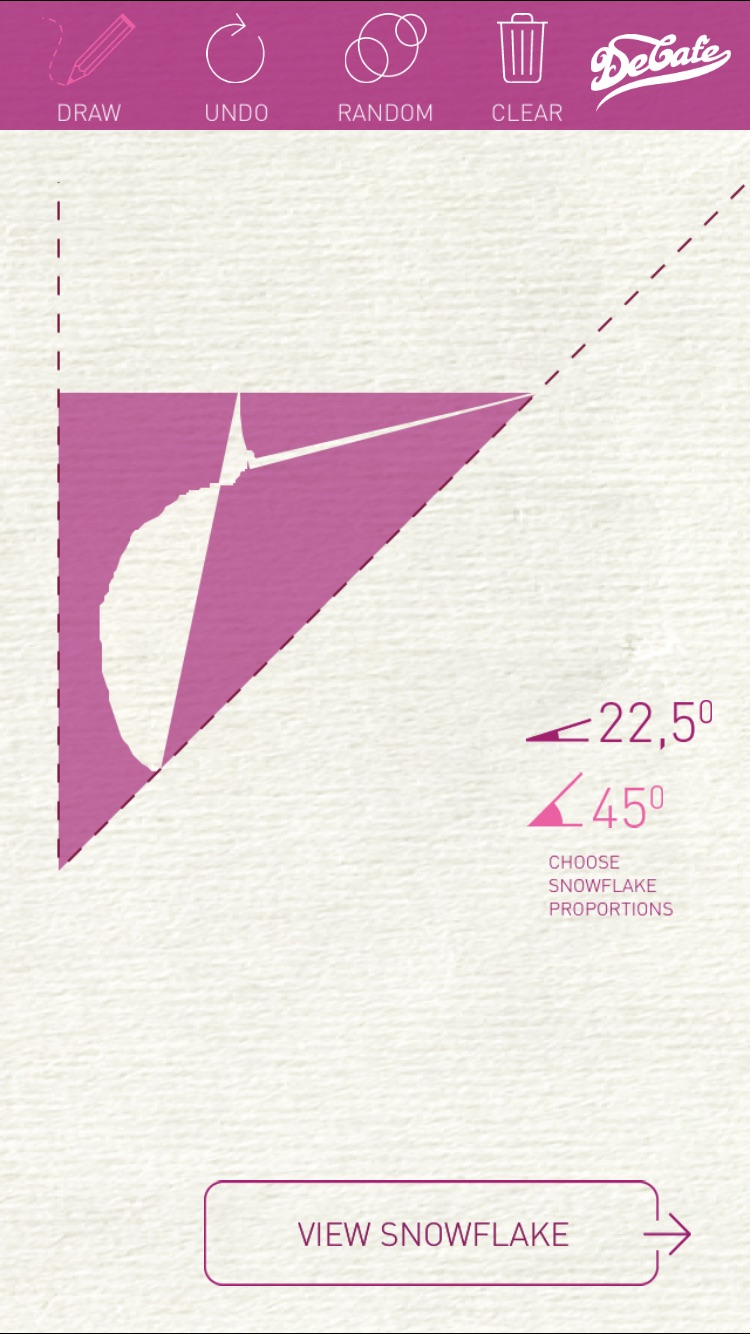
\includegraphics[width=0.7\linewidth]{Images/snowflakeCut}
                            \caption{The result of the free-form line drawn in \textbf{Figure~\ref{fig:snowflakeOutline}}. There is a bug in the application as this is not the cut the user would expect from what they have drawn.}
                            \label{fig:snowflakeCut}
                        \end{minipage}
                    \end{figure}
        
                \paragraph{Lessons Learned:}
                An application should be researched before it is made and assumptions checked - such as the assumption that was made about the dimensions of a snowflake. If the functionality of the buttons in the app is not working, there should be a response message from the application to inform the user as to what the problem is. Each button should have unique functionality. The cuts that are to be made in the virtual piece of paper should take up a large portion of the screen as this is the main area the user is interacting with.
            
            
            \subsubsection{Kirie}
            
                \paragraph{Type:} iPhone application 

                \paragraph{Description:}
                This application allows the user to draw lines on a virtual piece of paper which are transformed into cuts. The virtual piece of paper is unfolded. 

                \paragraph{Strengths:}
                The majority of the screen is used when creating the cut. This allows you to make intricate cuts and the overall feel of the app is minimalist and clean. 
                
                The option to load an image from the users library to cut from is available. 
                
                 \begin{wrapfigure}{r}{0.25\textwidth}
                    \centering
                    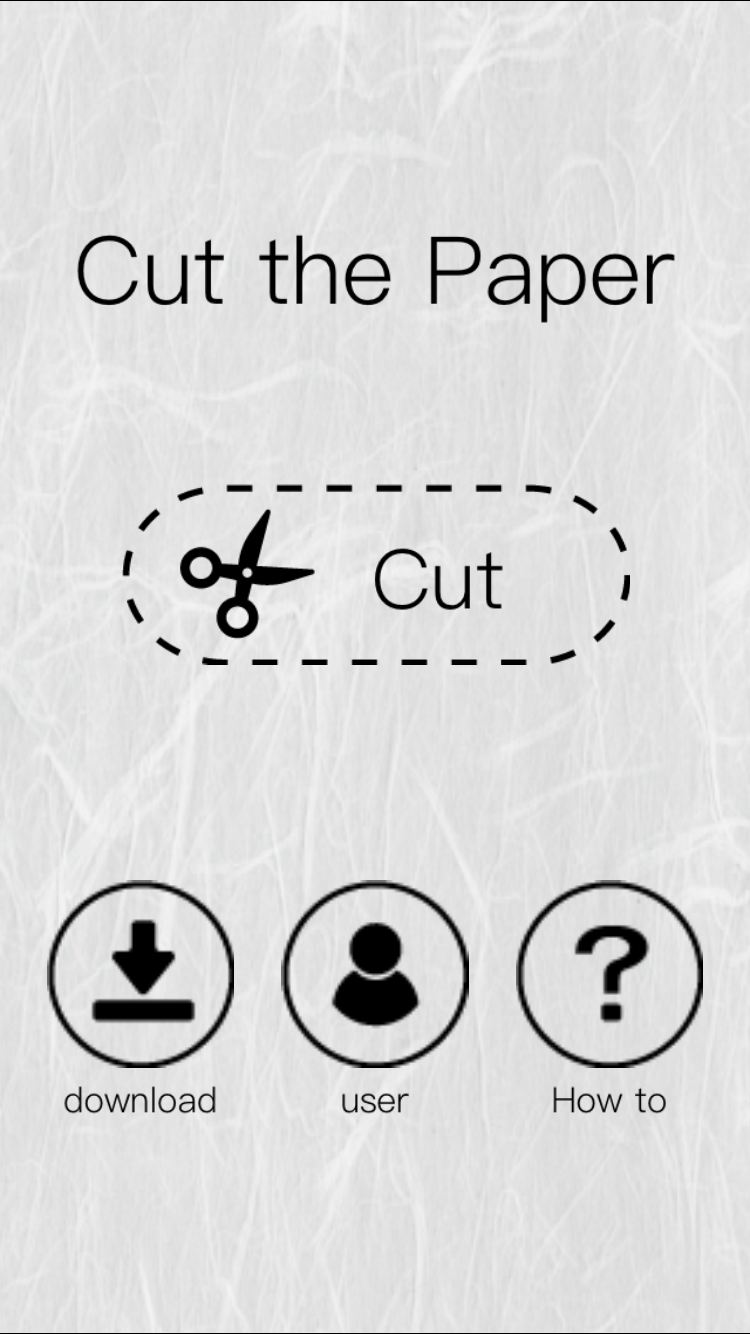
\includegraphics[width=0.25\textwidth]{Images/kirieMain.PNG}
                    \caption{aaaaa}
                    \label{fig:kirieMain}
                \end{wrapfigure}
                
                
                \paragraph{Weaknesses:}
                On the in initial screen (seen in \textbf{Figure~\ref{fig:kirieMain}}), only the "Cut" button works - which is also not a very clear button as it could be mistaken for a logo or image. If the download button is pressed, the app crashes and closes. If the "How to" button is pressed, there is no response from the app. If the user button is pressed, a pop up shows ups prompting a username. With any input the application closes the popup and returns to the same screen as before - there also appears no way to sign up or login. 
                
                On the finished cut screen shown in \textbf{Figure~\ref{fig:kirieCut}} the save icon button does not save the image anywhere despite a conformation pop-up. It is unclear what the functionality of the picture icon button is as the cuts have already been finalised. The upload icon results in a conformation pop-up (saying the image has been uploaded) but no upload has actually occurred. 
                
                The trace from the users finger is very sensitive and can result in cuts that are not smooth. The same shape cut e.g. the crosses created in \textbf{Figure~\ref{fig:kirieXs}} results in two cuts seen in \textbf{Figure~\ref{fig:kirieCut}} that are a) not consistent with cuts that would occur with a cutting knife or scissors, b) result in different cuts due to the starting point of each line. 
                
                The variety of tasks to do in the app is very limited.
                
                When the cuts are mirrored, the resolution of the image of the cuts decreases.
                
                \begin{figure}[!ht]
                        \begin{minipage}{0.45\textwidth}
                            \centering 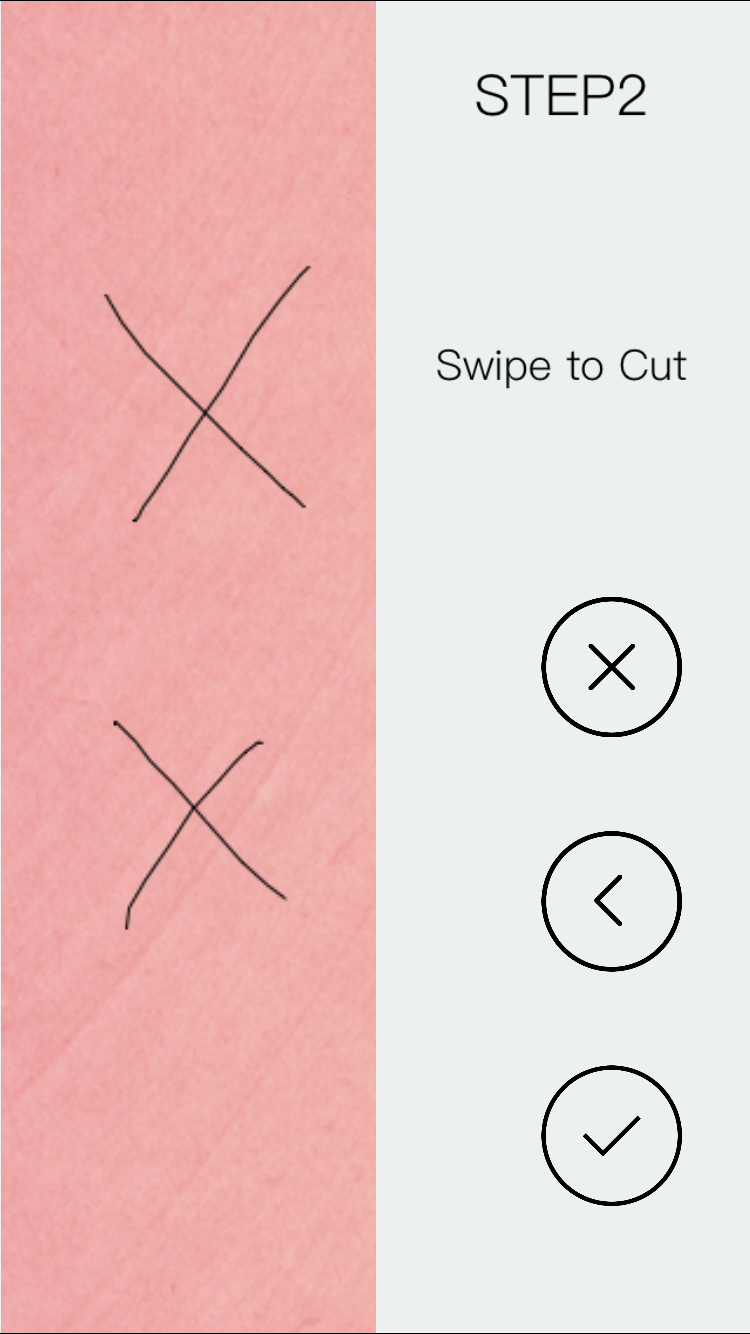
\includegraphics[width=0.7\linewidth]{Images/kirieXs.png}
                            \caption{aaaaa\\}
                            \label{fig:kirieXs}
                        \end{minipage}\hfill
                        \begin{minipage}{0.45\textwidth}
                            \centering
                            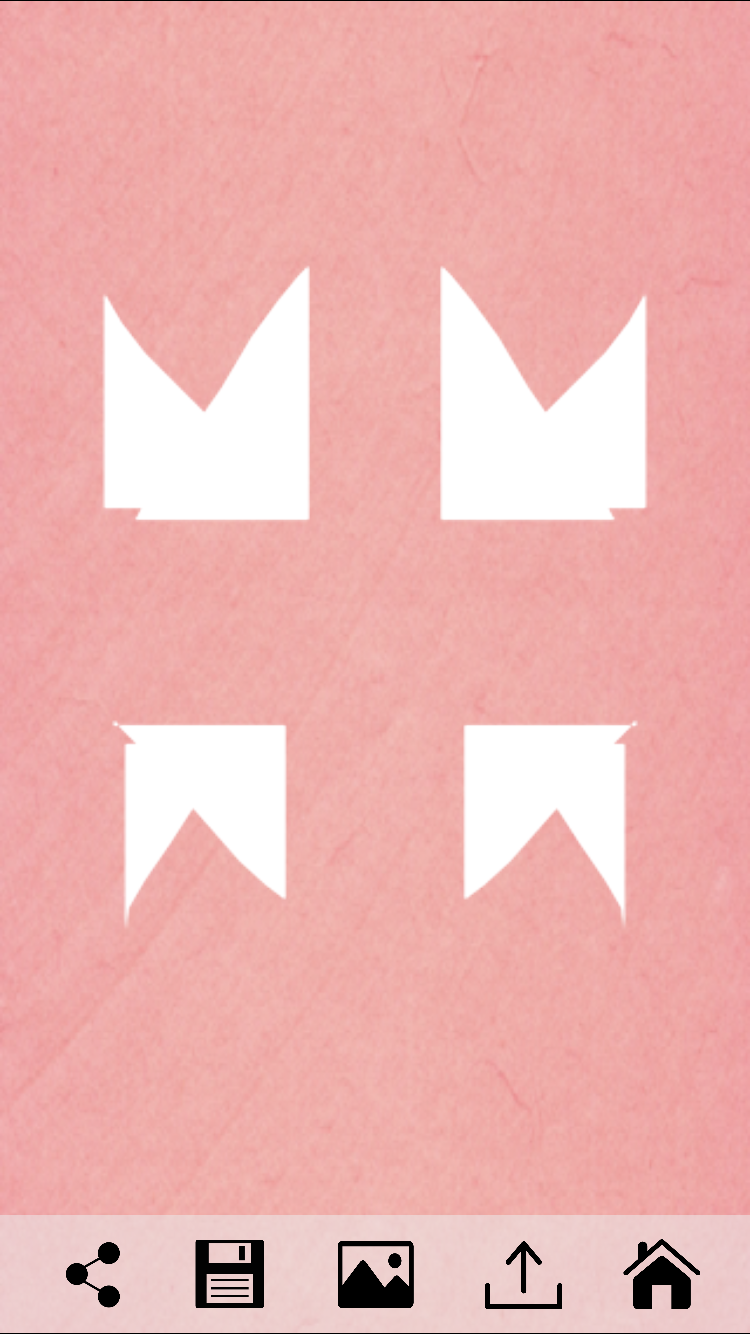
\includegraphics[width=0.7\linewidth]{Images/kirieCut.png}
                            \caption{The result of the free-form line drawn in . There is aaaa}
                            \label{fig:kirieCut}
                        \end{minipage}
                    \end{figure}
                
                \paragraph{Lessons Learned:}   
                A big portion of the screen allows the user to have more control and allows a greater space for creativity.
                
                The cuts created do not have to be closed shapes resulting in unexpected shapes being created after the user confirms the cut. 
               
                If the functionality of the buttons causes the application to crash, this is a major error and is unacceptable for any application. All buttons should be thoroughly tested throughout creation of my application. There could be conformation pop-ups in my application but only when the functionality works unlike in "kirie". 
                
                Additional features that add little to the app and are not completely necessary or relevant should not be implemented. Any non-core features should be added after the main functionality of the application works well.
                
                
                 \subsubsection{Handcraft Snowflakes}
            
                \paragraph{Type:} iPhone application 

                \paragraph{Description:}
                This application uses the character of Peppa Pig throughout. Peppa describes how to use the application which consists of cutting shapes out of a segment of a snowflake. There is gallery available where your snowflakes can be saved. Coins can be collected as snowflakes are made or purchased and can be redeemed for a new ready made shape to cut out the snowflake or to add a space in the gallery for another snowflake. 

                \paragraph{Strengths:}
                The theme is consistent through the use of a character.
                There are many language options so the character of Pepper Pig speaks in the language selected.
                In this case the snowflake has a reasonable number of sides. 

                \paragraph{Weaknesses:}
                After selection of a language, the language is inconsistent throughout the application. For example no matter which language you pick, the title for some sections - for example the colour picker - is always displayed in Russian. There is a black loading page before every screen displayed which stops the flow of the app and makes the app feel slow. This could be due to the many images displayed on screen. Glitches occur such as when selecting a colour, you ca still make cuts on the paper via the underlying view. 
                
                
                The main problem with the application is the assumed knowledge of the buttons. For example the undo buttons is usually what a back button is depicted as. On the snowflake cutting via free form screen, the arrow button is used as an undo button, but on the previous. On the snowflake cutting with pre-made shapes there is not an undo button. There is lack of consistency with the image of the button making use of the application unnecessarily complex screen the button used as a back button It is not clear what a lot of the buttons do. There is also the case of a lot of pop ups asking if you want to discard the current progress which seems excessive. 
                
                The adverts are very intrusive to the user experience even when on mute, the animation of Peppa pig still continues to animate speaking - however you cannot skip this section - the animation is rendered useless by the mute button however the application dose not register this. There are also no subtitles.
                
                The app will freeze if your cut touches itself. as seen in figure x. Sometimes when a cut is registered as a line it does not result in the paper being cut. 
                
                It is unclear what objects can be interacted with - on occasion there appears to be a glitch where the application indicates to the user an item should be touch --- figure--- however only the objects in figure --- respond to touch. 
                
                The name of the application is too long for the icon, therefore you cannot see the entire name of the app on iPhone screen. 
                
                \paragraph{Lessons Learned:}   
                
        \subsection{Cutting Paper Applications}
            \subsubsection{PaperCutCraft}
            
                \paragraph{Type:} iPhone application 
                 
                \paragraph{Description:} This application is for cutting paper

                \paragraph{Strengths:}
                There is a large amount of progression that can be had in the application with opportunity for
                
                \paragraph{Weaknesses:}
                While using the app, on occasion the cutting action stops working. The app creates a line representing a cut as usual, but it does not result in the paper being cut. After this occurs, there is no way to progress in the app even if the refresh button is used. There is another glitch where only the thin line drawn (e,g, figure a) is cut from the screen rather than the entire section of paper the user would expect to be cut from their trace as before. 
                It is unclear how to complete a level, the initial idea appear to cut but in order to get a score, you must press the forward triangle button "this is usually associated with a "play" feature which can be confusing to the user. 
                The shadow illusion can also be "cut off" breaking the illusion of the point of the shadow. 
                
                It is actually quite difficult to trace a thin line on this app as their finger is in the way
                
                The triangle button - the center button seen in fig a and b - means both finish the cut you are on, and move when the sa seen in figure c.  
                
                It is difficult to see what criteria there is for the accuracy rating as you use the aplication. 

                
                \paragraph{Lessons Learned:}
                
                \subsubsection{Topetope}
                 
                \paragraph{Type:} iPhone application 

                \paragraph{Description:}
                "TOPETOPE - cut the square" is an iPhone application that is advertised as a game where the user can cut a square piece of paper and there are cutting challenges that may come with time limits. The application did not appear to be working when tested multiple times with every effort made to troubleshoot it. Most of the application appeared to be inaccessible. 
                
                \paragraph{Strengths:}
                When the application does work (the initial screen shown in \textbf{Figure~\ref{fig:topeReality}} was somewhat functional), the cut of the paper is seamless. The user can drag their finger from one corner to another and the paper is cut along the line and one section falls off via an animation.
                
                \begin{figure}[!ht]
                        \begin{minipage}{0.45\textwidth}
                            \centering
                            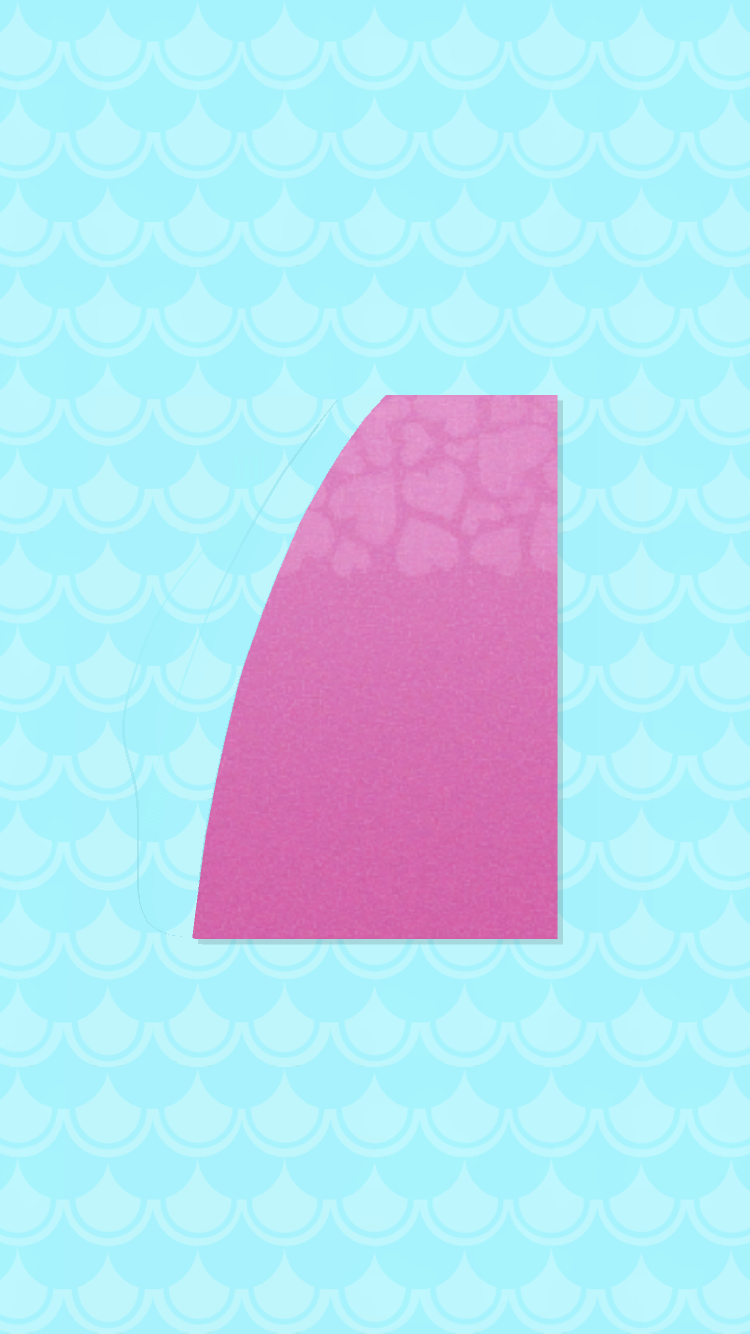
\includegraphics[width=0.6\linewidth]{Images/topeReality.png}
                            \captionsetup{margin = 0.5cm}
                            \caption{The initial (and only accessible) screen for the app Topetope. The user can use their finger to cut the piece of paper. The application responds approximately half the time. }
                            \label{fig:topeReality}
                        \end{minipage}
                        \begin{minipage}{0.48\textwidth}
                            \centering
                            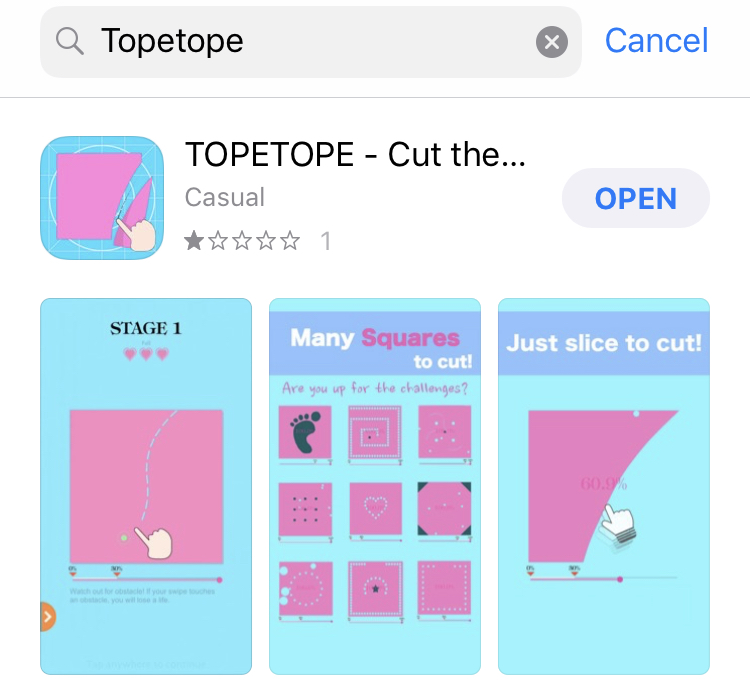
\includegraphics[width=0.85\linewidth]{Images/topeAdvertising.jpg}
                            \captionsetup{margin = 0.5cm}
                            \caption{The description for Topetope on the iPhone App Store.}
                            \label{fig:topeAdvertising}
                        \end{minipage}
                    \end{figure}
                    

                \paragraph{Weaknesses:}
                The application is extremely different to the advertised app as seen in figure \textbf{Figure~\ref{fig:topeAdvertising}}. In reality the user is only able to access one screen. With the level that can be accessed, it is unclear what the goal is.
                
                There is no home screen option, navigation available or the presence of tutorial page or directions. The cutting of the paper with the users finger only works approximately half the time.
                
                The glitching and lack of response from the app is very frustrating.
                
                
                There is no clear meaning of the word "topetope". May be translated from Spanish meaning the top or stop, however any translation of it does not particularly make sense in context. 
                
                 Topetope also lacked consistency as its description was different to the application.

                \paragraph{Lessons Learned:}
                In contrast to Topetope, the application I create should have a clear and obvious goal. A tutorial may be necessary as this would have been useful in this case. My application should be thoroughly tested at each stage and needs to reliably work throughout. This is especially important due to the relaxing mindfulness component of my application. Another aspect to consider is if the user is cutting the paper, with Topetope is not clear which side of the paper will be disappearing after it is cut. I need to make this decision clear if I am making it for the user, or allow the user to choose for themselves. 


       \subsection{Take home from reviewing other applications}
       
            \paragraph{}
            All of the iPhone applications I tested had inconsistencies with their main functionality of cutting shapes out of the segments / virtual paper. However the web application Paper Snowflake Maker did not have such an inconsistency. Whatever shape was drawn, the expected cut is created when the cut is finalised and when the unfolded virtual paper is revealed. The application I create should be consistent, reliable and the main feature of cutting should be easy to use.  
            
            Many of the examples had features which were either did not fully carry out the expected function or provided no response when interacted with. I will place importance on making sure every feature available work well and to the intended purpose over implementing many features. 
            
            None of the iPhone applications I looked at had a cut action that was consistent and worked reliably. All had some sort of glitch to do with the cut. The applications with a larger work space were nicer to use. 
            
            A few of the application had buttons where their intended functionality ambiguous, some where the same button actually changed functionality depending on the screen. If I choose to use icons, the action of the button should be apparent.
            
            Many of the applications reviewed had a snowflake / Christmas theme. Although this may be a good marketing tactic, I do not wish to restrict the kirigami to 3 folds (6 segments) and would like to make something diverse that is different to what is already available and not restricted to seasonal use. I also do not want to restrict the age range by creating a character like pepper pig. However I will try and extract the features that kept a coherent theme in that application.
            
            The size of the virtual paper should be large enough on the screen to allow for ease of interaction. The method which the user interacts with the paper should be simple and where the cut will occur should be clear (e.g. clear which part of the paper is cut - an inverted cut should be easy to carry out). 
            With a few of the application, another major flaw was that there is no clear goal or task. I should try to create an application where the goal or task is obvious.


\newpage
\section{Prototype}

    \subsection{Requirements}

        \paragraph{}

    \subsection{Target User}
    
            \paragraph{}
            

    \subsection{Wire Frames}
    Initially I created sketches of screen for the prototype and used the application "POP - Prototyping on Paper" to make the sketches interactive and test it out on potential users. %cite
    
        POP images

    Feedback
    
    Feedback I was given was that I needed to include undo and clear buttons for the creating images pages, 
    
    
    After collating the feedback, I translated the sketches to wireframes on balsamiq which I was familiar with as I used them on projects throughout the year. %https://balsamiq.com
    I kept in mind the requirements while creating the screens for the application.
\clearpage
             \begin{figure}
                \begin{minipage}[c]{0.35\textwidth}
                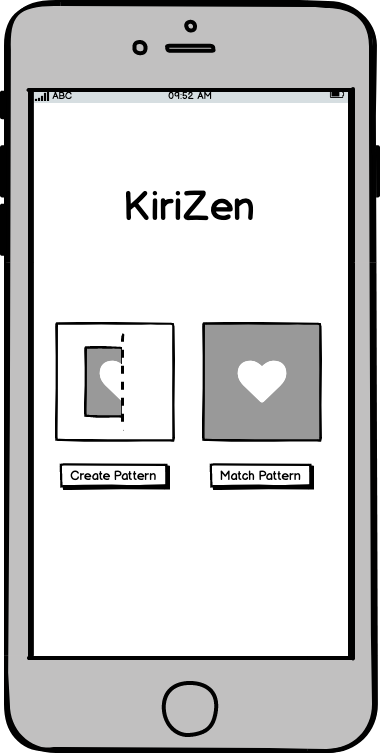
\includegraphics[width=1\textwidth]{Images/Prototype/prototypeHomeScreen.png}
                \end{minipage}\hfill
                \begin{minipage}[c]{0.65\textwidth}
                \captionsetup{font={normalsize}, margin = 1cm}
                \caption{The home screen will display the graphics for the two parts of the application - "Create Pattern" and "Match Pattern". The images used will display a pattern being created and a target image respectively. Clicking on the "Create Pattern" button will link the user to \textbf{Figure~\ref{fig:chooseFold}}, and clicking on match pattern will take the user to  \textbf{Figure~\ref{fig:target}}}
                \label{fig:homeScreen}
                \end{minipage}
            \end{figure}
            \begin{figure}
                \begin{minipage}[c]{0.65\textwidth}
                \captionsetup{font={normalsize}, margin = 1cm}
                \caption{This figure is where the user will be able to choose how they want their virtual piece of paper folded. The images for each button will show the virtual piece of paper folded in half, quarters, sixths and eights with straight edges. You cannot fold a piece of paper into odd numbers about a centre point which is why they are excluded here. The user will press one of these buttons which will link them to the corresponding version of the screen shown in \textbf{Figure~\ref{fig:createPattern}}}
                \label{fig:chooseFold}
                \end{minipage}\hfill
                \begin{minipage}[c]{0.35\textwidth}
                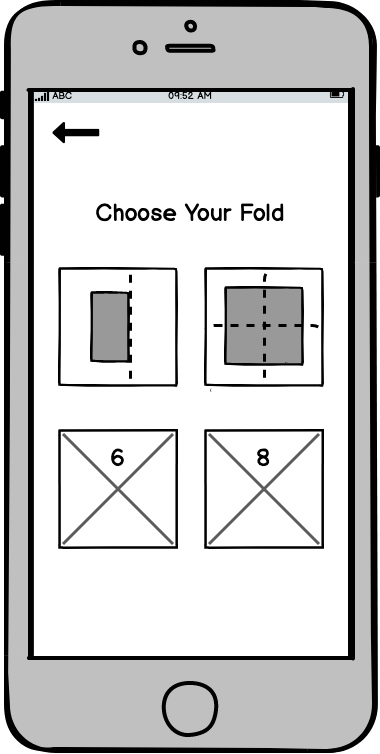
\includegraphics[width=1\textwidth]{Images/Prototype/prototypeChooseFold.png}
                \end{minipage}
            \end{figure}
            
            \begin{figure}
                \begin{minipage}[c]{0.35\textwidth}
                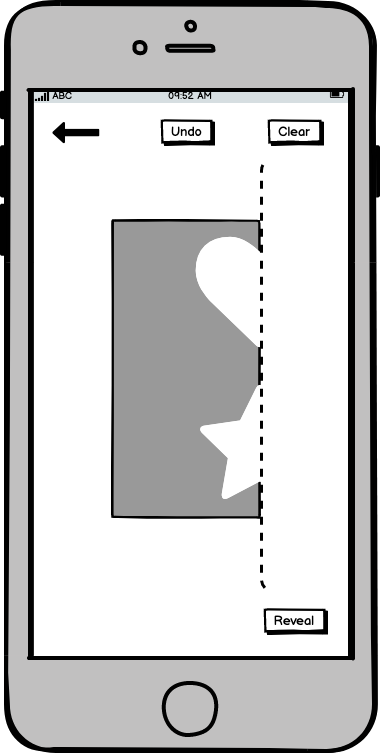
\includegraphics[width=1\textwidth]{Images/Prototype/prototypeCreatePattern.png}
                \end{minipage}\hfill
                \begin{minipage}[c]{0.65\textwidth}
                \captionsetup{font={normalsize}, margin = 1cm}
                \caption{The user will create the cuts from the virtually folded piece of paper on this screen. The shape of the folded segment displayed will depend on which button was pressed.
                They will have the option of deleting the last cut created with the "Undo" button, or refreshing the canvas with the "Clear" button.}
                \label{fig:createPattern}
                \end{minipage}
            \end{figure}
            
            \begin{figure}
                \begin{minipage}[c]{0.65\textwidth}
                \captionsetup{font={normalsize}, margin = 1cm}
                \caption{Caption}
                \label{fig:reveal}
                \end{minipage}\hfill
                \begin{minipage}[c]{0.35\textwidth}
                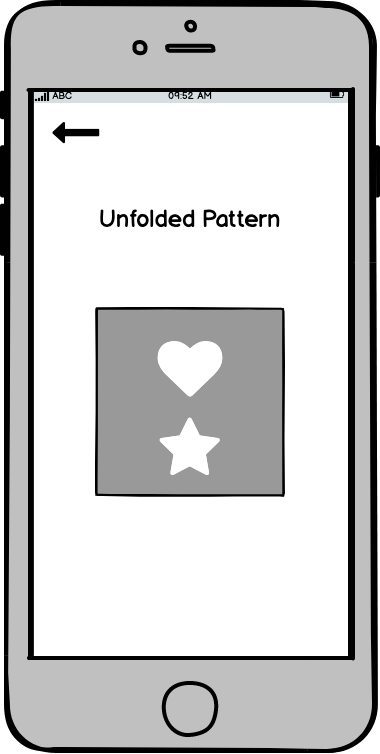
\includegraphics[width=1\textwidth]{Images/Prototype/prototypeReveal.png}
                \end{minipage}
            \end{figure}
            
           \begin{figure}
                \begin{minipage}[c]{0.35\textwidth}
                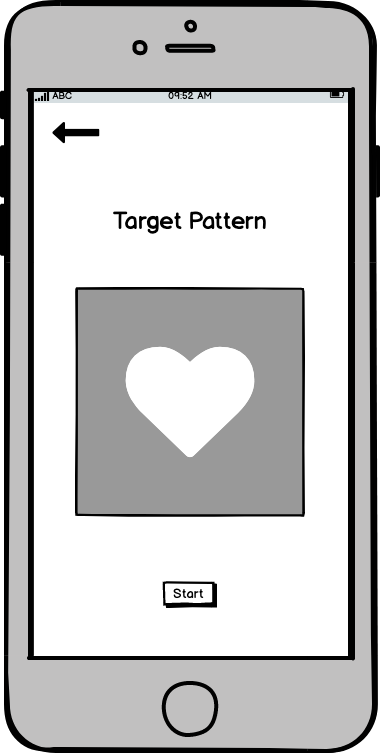
\includegraphics[width=1\textwidth]{Images/Prototype/prototypeTarget.png}
                \end{minipage}\hfill
                \begin{minipage}[c]{0.65\textwidth}
                \captionsetup{font={normalsize}, margin = 1cm}
                \caption{Caption}
                \label{fig:target}
                \end{minipage}
            \end{figure}
                           
           \begin{figure}
                \begin{minipage}[c]{0.65\textwidth}
                \captionsetup{font={normalsize}, margin = 1cm}
                \caption{Caption}
                \label{fig:matchPatternCreate}
                \end{minipage}\hfill
                \begin{minipage}[c]{0.35\textwidth}
                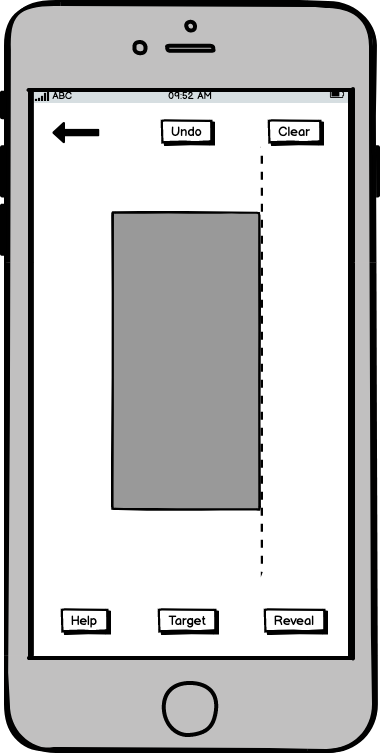
\includegraphics[width=1\textwidth]{Images/Prototype/prototypeMatchPatternCreate.png}
                \end{minipage}
            \end{figure}
                        \clearpage

            \begin{figure}
                \begin{minipage}[c]{0.35\textwidth}
                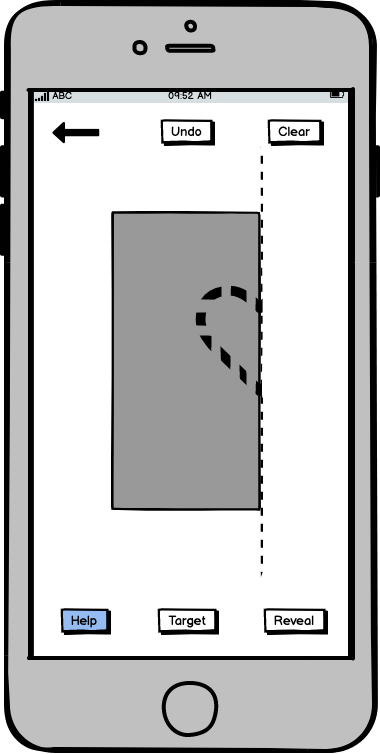
\includegraphics[width=1\textwidth]{Images/Prototype/prototypeMatchPatternCreateHelp.png}
                \end{minipage}\hfill
                \begin{minipage}[c]{0.65\textwidth}
                \captionsetup{font={normalsize}, margin = 1cm}
                \caption{Caption}
                \label{fig:matchPatternCreateHelp}
                \end{minipage}
            \end{figure}
            
            
                \paragraph{}
                Covergirl Covergirl
            

\newpage
\section{Creation of Software}

 
    \subsection{Layout}
    While creating the buttons I realised that they would be very small if layed out horizontally so I chose to lay them out vertically due to the long screen of the more recent iPhones.
    
            \paragraph{}

    \subsection{Creating Kirigami}
    
            \paragraph{}
        
        \subsubsection{Undo and Clear Functionality}
        
            \paragraph{} 
            After I incorporated this additional undo functionality I again observed the user interact with the application. 

    \subsection{Design choice}
    
            \paragraph{}

    \subsection{Reveal}
    
            \paragraph{}

        \subsubsection{Transformation}
        
                \paragraph{}

    \subsection{Inheritance}
    
            \paragraph{}

    \subsection{Target Shapes}
    
            \paragraph{}
            
    \subsection{Instructions}
    
        \paragraph{}

\newpage
\section{Human Computer Interaction}
%heuiristics
    \paragraph{}
    
        \subsection{Evaluation}
            
                \paragraph{} 

    \subsection{User Testing}
    
           \paragraph{} Throughout the project I asked my peers to test out the app and I observed how they interacted with it. 
        


    
    \subsection{Theme}
        
        \paragraph{}
        The name of the app is a combination of the words "kiri" and "zen". I checked to see if there were any apps with the same name or any applications or products however I did not come across anything of this name that was a similar product or any other product or concept that could potentially lead users elsewhere. If I did publish the application it would be easy for users to find and share. 

        \subsubsection{Additional Features}
        \paragraph{}
        The additional features of the application, while not crucial to the core function, are crucial to creating an overarching theme for the application creating a more complete experience for the user.    
        
         \subsubsection{Graphics}
    
        \begin{wrapfigure}{r}{0.25\textwidth}
                        \centering
                        
\includegraphics[width=0.25\textwidth]{KiriZen/icon.png}
                        \caption{Icon}
                        \label{fig:icon}
                    \end{wrapfigure}
            I created the icon in \textbf{Figure~\ref{fig:icon}} using the online tool canva %https://www.canva.com 
            to create the icon for the application. I chose a butterfly as they are symmetrical and the image
            
            I used the tool appicon %https://appicon.co
            to automatically generate the required images sized for different resolutions for different iPhone models. This is to allow the images to have the best possible resolution for the device it is being displayed on.  
            
            Need multiple sizes as the small components of the image – if downscaled from the large image would disappear when downscaled i.e. from 3x to 1x image. 
        
            I also used canva to create icons for all the buttons as  seen in fig x and y. I thought it was important to create the images from scratch rather than use stock images to make them personal to my app, so unlike some of the reviewed apps, the images are relevant and clearly relate to their function. I think it is also important to use original images to help create a uniqueness to my app, but in the case of the buttons on the main "creation" screens, it is more important that the functionality is clear than having an attractive icon which is why I generated the buttons from scratch with single words rather than inserting images into a button.
            
            I kept the colour palette consistent throughout and initially picking pastel colours for a calming modern  aura rather than saturated colours reminiscent from games from the 80s. I changed the navigation bar's colour to pink rather than the default blue to fit in with the colour scheme. 
    

                 \subsubsection{Launch Screen}
                I incorporated a loading screen while the application is starting up so the user can view a page that is relevant to the application rather than the default white page. This is especially important if the application is taking a long time to open - usually this happens on the initial load if the application is not already running in the background.
                
                 \subsubsection{Music Player}
                I have music playing in the background associated
                I added the music to enhance the mindfullness aspect of the application. As 
                
                %cite music
                
                 \subsubsection{Information Page and Launch Scree}
                
                The information page serves as additional insight for the user if they would like some additional information about the application. 


    \subsection{Deployment}
        \paragraph{}
        put on app store
        could do seasonal marketing if near Christmas -e.g. extra snowflake designs and animations
        
    
\newpage
\section{Discussion}
    \paragraph{}

    
    \subsection{Achievements}
    
        \paragraph{}
        Creating an application that unlike the other iPhone application has consistent, reliable and predictable cutting action. 
    
    \subsection{Challenges}
    
        \paragraph{}
        Deciding on how the user should cut. 
        
    \subsection{Architecture}
        
        \paragraph{}

        
    \subsection{Refactoring}
        
        \paragraph{}
        While creating 
            
\newpage
\section{Conclusion}

        \paragraph{}
    
        \subsection{Overall}
        
            \paragraph{}

        
        \subsection{Future}
        
                \paragraph{}
                
                Animation of folds
                
                Higher number of folds - 10, 12...
                
                Match pattern section
                Additional functionality could be added to the app such as an algorithm to generate random target images shaped but more sophisticated than randomly rendering shapes - some restrictions could apply such as shapes not touching - the variate of shapes etc.
                
                Algorithms for comparing target images to the image the user created 
                
                
                Wallpaper

        
\newpage
\let\Section\section 
\def\section*#1{\Section{#1}}  
\bibliographystyle{IEEEtran}
    \bibliography{bibliography}
    
\newpage
\Section{Appendix}
Download Xcode
        
% \begin{figure}[h!]
% \centering
% \includegraphics[scale=1.7]{universe}
% \caption{caption}
% \label{fig:nameof file}
% \end{figure}

\end{document}
